\documentclass{letter}
\usepackage{graphicx}
\usepackage{fullpage}
\signature{Adam J. Gray}


\begin{document}
\begin{letter}{The Hon. Joe Hockey M.P. \\ Level 6, 100 Mount Street \\ North Sydney 2059 NSW }

\opening{Mr Hockey,}

I am writing to you in regards to the budget you handed down for the 2014-15 financial year.

As a student, but more importantly, an Australian, I am dismayed and somewhat disgusted with this budget.
It attacks principles not only fundamental to the Australian way of life, 
but to any modern liberal democracy. It asks the poor to pay at lot more,
and the rich to pay only a little more. It disincentives education. It plays games with public health
and medical research and your budget also fails to properly address the complicated issue
of an aging population. 

Firstly, however, I would like to refute the idea that there is a ``budget emergency'' with
``ballooning levels of public debt''. 
I believe that this can be done in one graph.

\begin{centering}
	\ \ \ \ \ \ \ \ \ \ \ \ \ \ \ \ \ \ 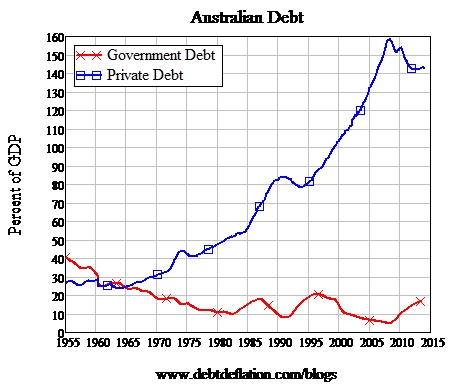
\includegraphics[scale=0.7]{public-private-debt}
\end{centering}

The idea that the budget is in such dire need of ``repair'', that you would need
to slash important social and economic programs is not based on fact. Either you are lying,
or you have been fed a lie and you have not done your job.


Almost everyone acknowledges that education will be a major key to success for individuals
in the 21st century, more so than ever before. By allowing universities to charge much higher fees,
while simultaneously reducing federal funding to universities, you are endangering the 
future of this country. Encumbering students with higher levels of debt, means that many 
students, especially those from lower socio-economic backgrounds will be deterred from university.

While you might argue that you are increasing funding to scholarships, I would argue that 
getting a scholarship is a tricky business and filled with uncertainty. I am lucky enough to
have been the recipient of a couple of small scholarships, but I am also lucky enough to have never
had to rely on a scholarship. If I had to, it's almost certain I would not be at university.

I believe that a student's access to education, and aspiration to achieve, should not
be limited by their parent's income. If we want Australia to be successful in the 21st century
we are going to need to be inclusive with education. It's too important of our future as a nation,
to simply let ``the market'' decide who gets an education.

While I think your changes to education are dangerous, I think your changes to health-care access
are disgusting. A seven dollar co-payment may not seem much to you, but to a child 
born into less fortunate circumstances, it's enough of a barrier to stop their parents taking
them to the doctor. You cannot value the health and wellbeing of children in ``middies of beer''.
That is disgusting, and an attack on the Australian ``fair go''.

You might argue that some of this money is being poured into a medical research fund, 
but with the cuts to education and the fees for research degrees,
who's going to be there to do the actual research? Further, why would you charge the sick more
to fund research programs that should be funded anyway? I understand that you need the 
revenue to run the research programs, but tax the general community, not specifically the sick. 
That's just heartless.

While I understand that Australia's aging population is a difficult issue that successive governments
have failed to address effectively, your approach is just policy laziness. It might be the case that with
improving health throughout the community, (something you are undermining), some people may be able
to effectively work into their 60s and 70s. This is not the case for everyone, especially manual
laborers. Also I don't believe that throwing ten thousand dollars at business is going to 
help the employment outcomes of older Australians.  

I understand that your changes to financial planning are technically not part of this
budget. I am dismayed, however, that you would remove the requirement for a financial planner
to work in the best interest of their client. This is especially important for older
Australians planning to rely on their superanuation. This is a ridiculous policy change
designed to allow financial institutions to rip off older Australians.

Until about a month ago I was not really involved in politics but now I am dedicating my time
to stopping this destruction of Australia's future. If you think 
that so many Australian's are going to fade quietly into the darkness while you steal our
hopes and our dreams, then you are mistaken. This isn't just about education, health-care or welfare. 
This is about Australia, and what it means to be Australian. I strongly urge you to reconsider this ill conceived
and malicious attack on Australian society. 


\closing{Sincerely,}

\end{letter}
\end{document}